\documentclass[11pt]{article}

\usepackage[margin=1in]{geometry}
\usepackage{amsmath}
\usepackage{amssymb}
\usepackage{graphicx}
\usepackage{booktabs}
\usepackage[colorlinks=true,linkcolor=blue,citecolor=blue,urlcolor=blue]{hyperref}
\usepackage{natbib}

\title{Chess as a Language: Tokenization, Rule Acquisition, and Emergent Board State in a Sub-500K-Parameter Transformer}
\author{Gregory Gestrin \\ \small Department of Applied Mathematics, University of California, Santa Cruz}
\date{\today}

\newcommand{\bpb}{\mathrm{bpb}}
\newcommand{\dd}[1]{\,\mathrm{d}#1}

\begin{document}

\maketitle

\begin{abstract}
\noindent
When an autoregressive transformer is trained purely by next-token prediction on a symbolic sequence domain, what does it actually learn: surface $n$-gram statistics, the syntactic rules of the formal language, or an internal representation of the underlying world state? We investigate this question by taking a from-scratch decoder-only transformer ($d_{\mathrm{model}}=64$, $L=5$ layers, $H=4$ heads, RoPE, RMSNorm, SwiGLU; $344\mathrm{K}$--$459\mathrm{K}$ parameters) written originally for natural-language modeling and training it without architectural modification on $72{,}885$ grandmaster chess games in canonical Standard Algebraic Notation (SAN). Holding the network architecture, training corpus, and compute budget fixed ($5{,}000$ optimizer steps, $256$-token context window), we sweep the byte-level Byte-Pair Encoding (BPE) vocabulary size across $V \in \{257, 512, 1024, 2048\}$, where $V=257$ corresponds to unmerged raw bytes plus a game-separator token. Across four evaluation axes---bits-per-byte compression, legal-move generation under token-healed sampling, linear probing of the residual stream for the $64$-square board state, and game-outcome prediction---we find three main results. First, at sub-$500\mathrm{K}$ parameter scale, larger BPE vocabularies systematically degrade both compression ($1.067$ to $1.158$ bits/byte) and legal-move generation ($60.6\%$ down to $38.8\%$ teacher-forced legality; $5.74$ down to $2.42$ consecutive free-running legal plies), even though $V=2048$ sees $3.55\times$ more game text per context window. Second, linear probes trained on intermediate residual-stream activations reconstruct the $64\times 13$ relative board state at $72.6\%$--$73.1\%$ accuracy ($33.8\%$--$35.8\%$ on occupied squares), substantially outperforming both an identically initialized untrained network ($64.6\%$--$66.3\%$ overall; $8.3\%$--$14.4\%$ occupied) and a per-square majority baseline ($63.5\%$ overall; $2.7\%$ occupied), with probe accuracy peaking in layers $2$--$4$ before declining at the final layer. Third, neither linear activation probes ($38.6\%$--$39.7\%$ accuracy) nor zero-shot language-model scoring matches a simple material-plus-Elo baseline ($55.3\%$ accuracy, $0.550$ macro-$F_1$) on three-way outcome prediction, and BPE boundary merges induce a severe token-count bias that collapses zero-shot mid-game scoring to a single class for $V \ge 512$.
\end{abstract}

\section{Introduction}
\label{sec:intro}

Autoregressive language models are trained on a deceptively simple objective: given a prefix of discrete tokens $x_{1:t}$, predict the conditional probability distribution $p_\theta(x_{t+1} \mid x_{1:t})$ over the next token. In natural language, evaluating whether a trained model has learned the structural rules of its domain rather than surface correlations is complicated by the absence of a formal referee; grammaticality and truth in English are graded and context-dependent. Formal sequence domains with deterministic transition rules remove this ambiguity. Chess, recorded in Portable Game Notation (PGN) via Standard Algebraic Notation (SAN), provides an exact, deterministic state machine: every move string either corresponds to a unique legal transition on the $8\times 8$ board or is illegal, and the complete latent state (piece placement, side to move, castling rights, en passant square) is a deterministic function of the move history \citep{toshniwal2022chess,karvonen2024chess}.

This exactness turns qualitative questions about sequence modeling into quantitative, falsifiable measurements. Specifically, when a small transformer reads move sequences such as
\begin{center}
\texttt{1.e4 e5 2.Nf3 Nc6 3.Bb5 a6 4.Ba4 Nf6 5.O-O Be7 ... 1-0}
\end{center}
as plain text without ever seeing a board representation or the rules of chess, we can ask four progressively deeper questions:
\begin{enumerate}
\item \textbf{Tokenization and compression:} How does the granularity of the byte-level BPE vocabulary $V \in \{257, 512, 1024, 2048\}$ affect byte-normalized cross-entropy (bits per byte) when the transformer backbone and compute budget are held strictly fixed?
\item \textbf{Syntactic and state-dependent rule acquisition:} How often does the model assign highest probability to a legal chess move on held-out grandmaster positions, how many consecutive legal plies can it play autonomously before its first illegal move, and how does rule adherence degrade from the opening into the middlegame and endgame?
\item \textbf{Emergent world state:} Does the residual stream encode an explicit linear representation of the $64$ board squares across depth, as observed in larger models trained on Othello \citep{li2023othello} and chess \citep{karvonen2024chess}, or can probe performance be explained by static square-occupancy priors and random projections?
\item \textbf{Value estimation (game outcome):} Can the model infer who is winning (White win \texttt{1-0}, Black win \texttt{0-1}, or draw \texttt{1/2-1/2}) from a move prefix, either via linear probes on its hidden states or zero-shot via next-token likelihoods, compared against domain baselines using material balance and player Elo ratings \citep{elo1978}?
\end{enumerate}

A central methodological constraint of this study is that the core machine-learning stack---\texttt{model.py}, \texttt{nn\_utils.py}, \texttt{training\_utils.py}, and \texttt{lr\_schedule.py}, originally implemented from scratch for a natural-language modeling course on TinyStories---is kept byte-for-byte unchanged apart from the package import path. All domain adaptation occurs in the data pipeline, tokenizer sweep, token-healed inference sampler, and post-hoc probing suite.

\section{Architecture and Mathematical Formulation}
\label{sec:architecture}

\subsection{Byte-level BPE tokenization and byte-normalized loss}
\label{sec:bpe}

Let $\Sigma_0 = \{0, 1, \dots, 255\}$ denote the base alphabet of raw UTF-8 bytes, augmented by a reserved special token $s_{\mathrm{game}} = \texttt{<|game|>}$ that separates distinct games in the corpus and is never split or merged across boundaries. Byte-level Byte-Pair Encoding \citep{sennrich2016,radford2019} constructs a vocabulary $\mathcal{V}_V$ of size $V = 257 + M$ by starting from $\mathcal{V}_{257} = \Sigma_0 \cup \{s_{\mathrm{game}}\}$ and iteratively applying $M$ greedy merge rules. At step $m \in \{1, \dots, M\}$, the most frequent adjacent token pair $(u^\ast, v^\ast)$ in the training corpus (breaking ties deterministically by lexicographic pair order) is replaced by a new token $w_m = u^\ast \circ v^\ast$.

At $V=257$ ($M=0$), no merges occur: every character in canonical SAN (\texttt{e}, \texttt{4}, \texttt{N}, \texttt{f}, \texttt{3}, space, period) is its own token. As $V$ increases to $512$, $1024$, and $2048$, the tokenizer absorbs frequent domain substrings---first destination squares (\texttt{e4}, \texttt{f3}, \texttt{c6}), then full moves with punctuation (\texttt{Nf3}, \texttt{O-O}), and eventually multi-token sequences that straddle move boundaries (such as \texttt{"4 6.N"} or \texttt{".Rd1 R"}). To make training on a $96\,\mathrm{MB}$ corpus practical, we replace the naive Python loop over token pairs with a vectorized NumPy implementation (\texttt{chesslm.tokenizer}) that updates pair counts via masked array indexing; in unit tests across $40$ randomized corpora, it produces merge tables and token ID sequences bit-for-bit identical to the reference implementation at a ${\sim}35\times$ speedup.

Because a larger vocabulary packs more bytes into each token, raw per-token cross-entropy $\mathcal{L}_{\mathrm{tok}}(\theta)$ (in nats/token) increases with $V$ even when the underlying probability distribution over byte strings improves. Let $N_{\mathrm{bytes}}$ and $N_{\mathrm{tok}}(V)$ denote the total byte length and token count of the held-out validation split under vocabulary $V$, and define the empirical compression ratio
\begin{equation}
\rho(V) = \frac{N_{\mathrm{bytes}}}{N_{\mathrm{tok}}(V)} \quad \text{(bytes per token)}.
\label{eq:bpt}
\end{equation}
By the chain rule of probability over deterministic prefix encodings, the negative log-likelihood normalized per byte and converted to base-$2$ bits is
\begin{equation}
\bpb(\theta; V) = \frac{\mathcal{L}_{\mathrm{tok}}(\theta)}{\rho(V)\,\ln 2}.
\label{eq:bpb}
\end{equation}
All cross-vocabulary comparisons in Section~\ref{sec:results} use $\bpb(\theta; V)$ from Equation~\eqref{eq:bpb}. Conversely, for a fixed sequence length of $T = 256$ tokens, the effective horizon of game text visible to self-attention scales linearly with $\rho(V)$:
\begin{equation}
C_{\mathrm{bytes}}(V) = T\,\rho(V).
\label{eq:cbytes}
\end{equation}

\subsection{Decoder-only transformer backbone}
\label{sec:transformer}

Given a token sequence $x = (x_1, \dots, x_T) \in \{0, \dots, V-1\}^T$, the model maps $x$ to a sequence of residual-stream states $h^{(0)}, h^{(1)}, \dots, h^{(L)} \in \mathbb{R}^{T \times d_{\mathrm{model}}}$. The initial state is the token embedding $h^{(0)}_t = W_E[x_t]$, where $W_E \in \mathbb{R}^{V \times d_{\mathrm{model}}}$. Each transformer block $\ell \in \{1, \dots, L\}$ applies pre-normalization via Root Mean Square Layer Normalization \citep{zhang2019rmsnorm}:
\begin{equation}
\mathrm{RMSNorm}(u) = \frac{u}{\sqrt{\frac{1}{d_{\mathrm{model}}}\sum_{i=1}^{d_{\mathrm{model}}} u_i^2 + \varepsilon}} \odot \gamma,
\label{eq:rmsnorm}
\end{equation}
where $\varepsilon = 10^{-5}$ and $\gamma \in \mathbb{R}^{d_{\mathrm{model}}}$ is a learned gain vector.

In causal multi-head self-attention \citep{vaswani2017} with $H$ heads of dimension $d_k = d_{\mathrm{model}}/H$, the normalized state $\tilde{h} = \mathrm{RMSNorm}(h^{(\ell-1)})$ is projected into queries, keys, and values $Q, K, V_{\mathrm{val}} \in \mathbb{R}^{H \times T \times d_k}$. Relative positional information is injected via Rotary Position Embeddings \citep[RoPE;][]{su2024rope}: for head index $h$, token position $t \in \{0, \dots, T-1\}$, and coordinate pair $(2j, 2j+1)$ with $j \in \{0, \dots, d_k/2 - 1\}$, the two-dimensional subspace is rotated by angle $t\theta_j$, where $\theta_j = 10000^{-2j/d_k}$:
\begin{equation}
\begin{pmatrix} q'_{t,2j} \\ q'_{t,2j+1} \end{pmatrix}
=
\begin{pmatrix} \cos(t\theta_j) & -\sin(t\theta_j) \\ \sin(t\theta_j) & \cos(t\theta_j) \end{pmatrix}
\begin{pmatrix} q_{t,2j} \\ q_{t,2j+1} \end{pmatrix},
\label{eq:rope}
\end{equation}
and identically for $K$. Because $R(t\theta_j)^\top R(s\theta_j) = R((s-t)\theta_j)$, the inner product $\langle q'_t, k'_s \rangle$ depends only on the relative token offset $t - s$. The attention weights for layer $\ell$ and head $h$ are
\begin{equation}
A^{(\ell, h)}_{t, s} = \frac{\exp\!\left(\langle q'_t, k'_s \rangle / \sqrt{d_k} + M_{t,s}\right)}{\sum_{s'=0}^{T-1} \exp\!\left(\langle q'_t, k'_{s'} \rangle / \sqrt{d_k} + M_{t,s'}\right)},
\qquad
M_{t,s} = \begin{cases} 0 & \text{if } s \le t, \\ -\infty & \text{if } s > t, \end{cases}
\label{eq:attn}
\end{equation}
and the block update is followed by a position-wise SwiGLU feed-forward network \citep{shazeer2020glu}:
\begin{align}
a^{(\ell)} &= h^{(\ell-1)} + W_O\,\mathrm{Concat}_{h=1}^H\!\left(A^{(\ell,h)} V_{\mathrm{val}}^{(h)}\right), \label{eq:res1} \\
\mathrm{FFN}(u) &= W_{\mathrm{down}}\!\left(\mathrm{SiLU}(W_{\mathrm{gate}} u) \odot (W_{\mathrm{up}} u)\right), \qquad \mathrm{SiLU}(z) = \frac{z}{1 + e^{-z}}, \label{eq:swiglu} \\
h^{(\ell)} &= a^{(\ell)} + \mathrm{FFN}\!\left(\mathrm{RMSNorm}(a^{(\ell)})\right). \label{eq:res2}
\end{align}
After layer $L$, a final $\mathrm{RMSNorm}$ is applied and projected to vocabulary logits via weight tying with the input embedding matrix, $z_t = \mathrm{RMSNorm}(h^{(L)}_t) W_E^\top \in \mathbb{R}^V$.

\paragraph{Parameter budget.} Because all linear projections and RMSNorm layers are bias-free and the output head is tied to $W_E$, the exact deduplicated parameter count is
\begin{equation}
P(V) = \underbrace{V d_{\mathrm{model}}}_{\text{tied embedding}} + L\Bigl(\underbrace{4 d_{\mathrm{model}}^2}_{\text{attention } Q,K,V,O} + \underbrace{3 d_{\mathrm{model}} d_{\mathrm{ff}}}_{\text{SwiGLU FFN}} + \underbrace{2 d_{\mathrm{model}}}_{\text{block RMSNorms}}\Bigr) + \underbrace{d_{\mathrm{model}}}_{\text{final RMSNorm}}.
\label{eq:params}
\end{equation}
For the base configuration ($d_{\mathrm{model}}=64$, $L=5$, $H=4$, $d_{\mathrm{ff}}=256$), the non-embedding transformer body contains exactly $327{,}680$ parameters ($5 \times (16{,}384 + 49{,}152 + 128) - 64$ plus the final norm, totaling $5 \times 65{,}536 + \text{norms}$). Specifically, $4d_{\mathrm{model}}^2 + 3d_{\mathrm{model}}d_{\mathrm{ff}} = 16{,}384 + 49{,}152 = 65{,}536$ per layer ($327{,}680$ across $5$ layers), and with the embedding table $64V$ the total parameter count ranges from $344{,}128$ at $V=257$ ($4.8\%$ in embeddings) to $458{,}752$ at $V=2048$ ($28.6\%$ in embeddings), staying strictly below the $500{,}000$-parameter course budget across all runs.

\subsection{Token-healed move sampling}
\label{sec:healing}

A subtle failure mode arises when evaluating a BPE-trained model on move generation. Suppose the game has reached ply $k$ and we prompt the model to generate ply $k+1$ by feeding the string prefix $\pi_k$, such as \texttt{"1.e4 e5 2."}. In training, the model never saw the trailing characters \texttt{" 2."} at the end of a sequence; instead, those characters were always followed immediately by a move such as \texttt{"Nf3"}, and for $V \ge 512$ the BPE tokenizer often merges across that boundary (for instance, merging \texttt{"2.N"} into a single token). Naively encoding $\pi_k$ forces a token boundary right before the move, presenting the model with an out-of-distribution token sequence and artificially depressing its legal-move rate.

To eliminate this boundary artifact, \texttt{chesslm.legality.Sampler} implements \emph{token healing}:
\begin{enumerate}
\item Encode the prompt $\pi_k$ into tokens $(t_1, \dots, t_{m-1}, t_m)$, strip the final token $t_m$, and record its byte string $b^\ast = \mathrm{bytes}(t_m)$.
\item Autoregressively sample from the prefix $(t_1, \dots, t_{m-1})$, but at each decoding step mask the vocabulary logits to $-\infty$ for any candidate token $w \in \mathcal{V}_V$ whose byte string is incompatible with the unconsumed prefix of $b^\ast$ (i.e., neither a prefix of the remaining bytes of $b^\ast$ nor starting with the remaining bytes of $b^\ast$).
\item Once the generated bytes cover $b^\ast$, remove the constraint and continue decoding until a whitespace or game-termination delimiter is emitted, then strip $b^\ast$ to recover the newly generated SAN move string.
\end{enumerate}
We verify this algorithm mathematically and empirically in \texttt{tests/test\_legality.py}: an oracle model that assigns high logit to the true token sequence of a game achieves $100\%$ legal-move rate and $100\%$ exact-match rate at every ply under token healing, whereas naive unhealed prompting fails whenever a BPE merge crosses the prompt boundary.

\subsection{Residual-stream alignment and linear probes}
\label{sec:probing-math}

To test whether the model maintains an internal representation of the chess board, we attach linear classifier probes \citep{alain2017probes} to the residual stream. Because BPE tokens do not align one-to-one with chess moves, feature extraction must be anchored in byte coordinates. Let $e_k \in \mathbb{N}$ denote the exact byte offset where the $(k+1)$-th move string ends in the canonical game movetext. For an encoded token sequence $(x_1, \dots, x_T)$ with cumulative byte lengths $c_i = \sum_{j=1}^i |\mathrm{bytes}(x_j)|$, we locate the unique token index
\begin{equation}
\tau(k) = \min\{\, i \in \{1, \dots, T\} : c_i \ge e_k \,\},
\label{eq:tau}
\end{equation}
which is the exact token step at which the model has just finished reading move $k$ (and no bytes from move $k+2$ if a boundary merge includes the trailing space). At position $\tau(k)$, we extract the layer-$\ell$ activation vector $h^{(\ell)}_{\tau(k)} \in \mathbb{R}^{d_{\mathrm{model}}}$ for $\ell \in \{0, 1, \dots, L\}$, where $\ell=0$ is the raw token embedding $h^{(0)}$ and $\ell=L$ is the post-final-RMSNorm state.

\paragraph{Board-state probe ($64$ squares $\times$ $13$ classes).} After move $k$, let $B_k$ be the true board position reconstructed by replaying the first $k+1$ moves in \texttt{python-chess}. Each square $s \in \{0, \dots, 63\}$ (from \texttt{a1} $= 0$ to \texttt{h8} $= 63$) is assigned a class label $y_{k,s} \in \{0, 1, \dots, 12\}$. We evaluate two labeling conventions:
\begin{itemize}
\item \emph{Absolute}: class $0$ is empty, classes $1$--$6$ are White ($\mathrm{P, N, B, R, Q, K}$), and classes $7$--$12$ are Black ($\mathrm{p, n, b, r, q, k}$).
\item \emph{Relative to the mover}: class $0$ is empty, classes $1$--$6$ belong to the side that just moved, and classes $7$--$12$ belong to the opponent.
\end{itemize}
Given $N$ training positions with standardized feature matrix $\tilde{X}^{(\ell)} \in \mathbb{R}^{N \times d_{\mathrm{model}}}$ (zero mean and unit variance per coordinate on the training split), we fit $64$ independent multinomial logistic regression heads with weights $W^{(\ell)}$ and biases $b^{(\ell)}$ of shape $d_{\mathrm{model}} \times 64 \times 13$ and $64 \times 13$ by minimizing the $\ell_2$-regularized cross-entropy
\begin{equation}
\mathcal{J}_{\mathrm{board}}(W^{(\ell)}, b^{(\ell)}) = -\frac{1}{64N}\sum_{n=1}^N \sum_{s=0}^{63} \ln \mathrm{softmax}\!\left(\tilde{x}_n^\top W^{(\ell)}_s + b^{(\ell)}_s\right)_{y_{n,s}} + \lambda \|W^{(\ell)}\|_F^2
\label{eq:probe-loss}
\end{equation}
with $\lambda = 10^{-3}$ for $300$ full-batch Adam epochs ($\text{lr}=0.05$). Because a majority of squares on a chessboard are empty mid-game (making overall accuracy artificially high even for trivial predictors), we separately report \emph{occupied-square accuracy}, conditioned on $y_{n,s} \neq 0$, and compare against two mandatory controls: (i) the identical probe architecture fit on activations from a randomly initialized, \emph{untrained} copy of the transformer, and (ii) a per-square majority-class baseline.

\paragraph{Attention collapse from tokens to moves.} To inspect what the attention heads look back at in chess terms (\texttt{chesslm.attention}), we assign each token $i$ to the move index $m(i) = \min\{\,k : e_k > c_{i-1}\,\}$ that owns its first byte. For query move $q$ (read at token $\tau(q)$) and earlier key move $k \le q$, the move-level attention matrix is obtained by summing token attention over all tokens owned by move $k$:
\begin{equation}
\bar{A}^{(\ell, h)}_{q, k} = \sum_{s : m(s) = k} A^{(\ell, h)}_{\tau(q), s}.
\label{eq:move-attn}
\end{equation}
Because $\{\,s : m(s) = k\,\}_{k=0}^q$ partitions the causal prefix $\{0, \dots, \tau(q)\}$, the move-level weights satisfy $\sum_{k=0}^q \bar{A}^{(\ell, h)}_{q, k} = 1$ for every query move $q$.

\section{Dataset and Experimental Protocol}
\label{sec:protocol}

\subsection{Grandmaster PGN corpus and canonicalization}

Raw PGN archives for $19$ world-class players (Anand, Aronian, Capablanca, Carlsen, Caruana, Ding, Firouzja, Fischer, Giri, Grischuk, Karpov, Kasparov, Kramnik, Nakamura, Nepomniachtchi, Rapport, So, Tal, and Topalov) were collected from \texttt{pgnmentor.com}. Across all files, $82{,}102$ raw game records were parsed. Because games between two players in the list appear in both archives, and because historical PGN files contain occasional corrupted move strings or non-standard starting positions (\texttt{FEN}/\texttt{SetUp} headers), every game was replayed from the standard initial board in \texttt{python-chess}. Games with fewer than $2$ plies, non-standard starts, or illegal SAN moves ($26$ games total) were rejected, and every valid move was re-rendered via \texttt{board.san(move)} into a single canonical format (\texttt{"1.e4 e5 2.Nf3 Nc6 ... 1-0"}).

De-duplicating by exact canonical movetext removed $9{,}191$ duplicate games, leaving $72{,}885$ unique, verified grandmaster games. Using a fixed pseudorandom permutation (seed $42$), games were partitioned at the game level into $96\%$ training ($69{,}971$ games), $2\%$ validation ($1{,}457$ games), and $2\%$ test ($1{,}457$ games), guaranteeing zero game-level leakage across splits.

\subsection{Controlled vocabulary sweep and probing setup}

All four models ($V \in \{257, 512, 1024, 2048\}$) were trained on an NVIDIA Tesla T4 GPU under identical hyperparameters (\texttt{configs/base.yaml}): $d_{\mathrm{model}}=64$, $L=5$, $H=4$, $d_{\mathrm{ff}}=256$, dropout $0.0$, context length $T=256$, batch size $32$, AdamW \citep{loshchilov2019adamw} with $\beta_1=0.9$, $\beta_2=0.95$, weight decay $0.1$, gradient norm clipping at $1.0$, and a cosine learning-rate schedule with linear warmup over $200$ steps to $\eta_{\max}=10^{-3}$ decaying to $\eta_{\min}=10^{-5}$ at step $5{,}000$. Each training run required $290$--$318$ seconds (${\approx}5$ minutes) on the T4.

Rule acquisition was evaluated on the held-out test split via two metrics: (i) teacher-forced legality over $500$ randomly sampled game prefixes (stratified into opening $\text{ply} < 20$, middlegame $20 \le \text{ply} < 60$, and endgame $\text{ply} \ge 60$), and (ii) free-running rollouts on $50$ test games where the model is prompted with the first $10$ plies and plays both White and Black greedily ($T_{\mathrm{samp}}=0$) until its first illegal move or game termination (up to $60$ plies).

For the probing suite (\texttt{scripts/run\_probes.py}), $8$ plies per game were sampled from $4{,}000$ training games ($N_{\mathrm{train}} = 31{,}999$ positions) and all $1{,}457$ test games ($N_{\mathrm{test}} = 11{,}656$ positions). Outcome prediction (\texttt{1-0}, \texttt{0-1}, \texttt{1/2-1/2}) was evaluated across four game-progress quartiles ($0$--$25\%$, $25$--$50\%$, $50$--$75\%$, $75$--$100\%$ of total game length) comparing: (a) training-split majority class, (b) multinomial logistic regression on standard piece-value material balance $(1, 3, 3, 5, 9)$ and total piece count, (c) material balance augmented with normalized player rating difference $(\mathrm{Elo}_W - \mathrm{Elo}_B)/400$, (d) the best linear probe on residual-stream activations, and (e) zero-shot language-model log-likelihood scoring over $2{,}000$ test prefixes.

\section{Results}
\label{sec:results}

\subsection{Tokenization sweep: why raw bytes beat BPE at small scale}
\label{sec:res-sweep}

Table~\ref{tab:sweep} and Figures~\ref{fig:learning-curves}--\ref{fig:sweep-summary} summarize the vocabulary sweep. As intended, increasing $V$ from $257$ to $2048$ compresses the PGN text by $3.55\times$, expanding the effective context window from $260$ bytes (roughly $18$--$20$ plies) to $921$ bytes (roughly $65$--$70$ plies, often an entire game). Despite seeing $3.55\times$ more bytes per batch and per context window, larger vocabularies perform monotonically worse on validation bits per byte ($1.067$ at $V=257$ vs.\ $1.158$ at $V=2048$) and substantially worse on downstream chess metrics.

\begin{table}[htbp]
\centering
\caption{Controlled BPE vocabulary sweep on $72{,}885$ grandmaster games ($5{,}000$ steps, $d_{\mathrm{model}}=64$, $L=5$, $H=4$, $T=256$). Lower bits/byte is better; higher legality and exact match are better.}
\label{tab:sweep}
\medskip
{\footnotesize\setlength{\tabcolsep}{4.5pt}
\begin{tabular}{@{}rrrrrrrrr@{}}
\toprule
Vocab $V$ & Params & Embed $\%$ & Bytes/tok & Context (B) & Val nats/tok & Val bpb $\downarrow$ & Legal rate $\uparrow$ & Free plies $\uparrow$ \\
\midrule
$257$  & $344{,}128$ & $4.8\%$  & $1.014$ & $260$ & $0.750$ & $\mathbf{1.067}$ & $\mathbf{0.606}$ & $\mathbf{5.74}$ \\
$512$  & $360{,}448$ & $9.1\%$  & $2.372$ & $607$ & $1.795$ & $1.092$ & $0.518$ & $4.68$ \\
$1024$ & $393{,}216$ & $16.7\%$ & $2.999$ & $768$ & $2.360$ & $1.135$ & $0.538$ & $3.56$ \\
$2048$ & $458{,}752$ & $28.6\%$ & $3.597$ & $921$ & $2.887$ & $1.158$ & $0.388$ & $2.42$ \\
\bottomrule
\end{tabular}
}
\end{table}

\begin{figure}[htbp]
\centering
\IfFileExists{../figures/fig1_learning_curves_bpb.png}{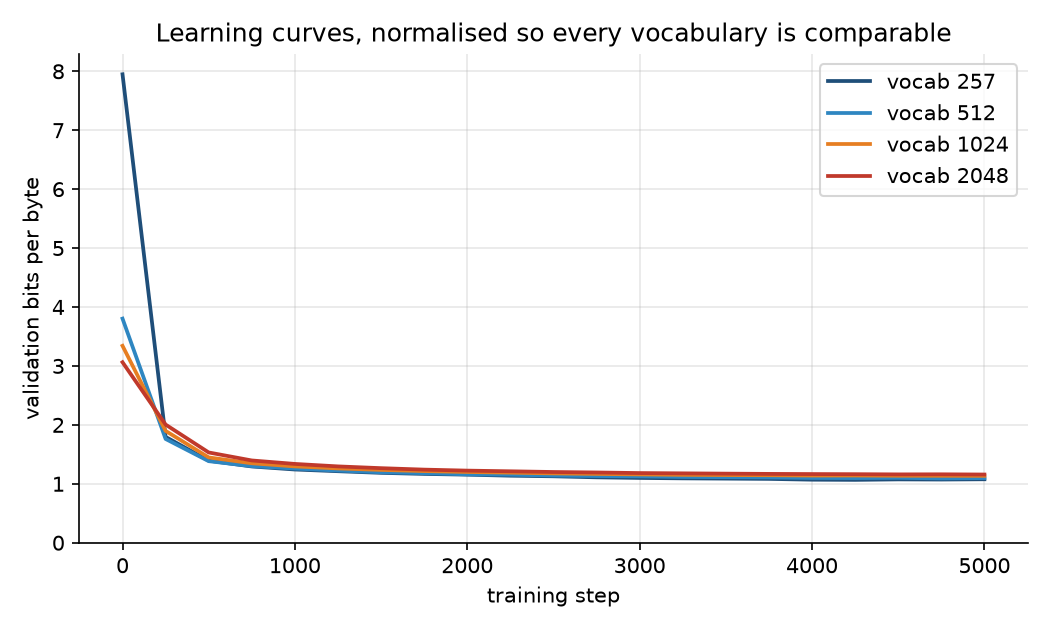
\includegraphics[width=0.78\textwidth]{../figures/fig1_learning_curves_bpb.png}}{\typeout{Missing figure: fig1_learning_curves_bpb.png}}
\caption{Validation learning curves normalized to bits per byte (Equation~\ref{eq:bpb}) across the $5{,}000$-step training run. Although larger vocabularies start at lower initial loss due to unigram token frequencies, the byte-level model ($V=257$) crosses below all BPE models within the first $500$ steps and maintains the lowest validation bits per byte throughout training.}
\label{fig:learning-curves}
\end{figure}

\begin{figure}[htbp]
\centering
\IfFileExists{../figures/fig2_sweep_summary.png}{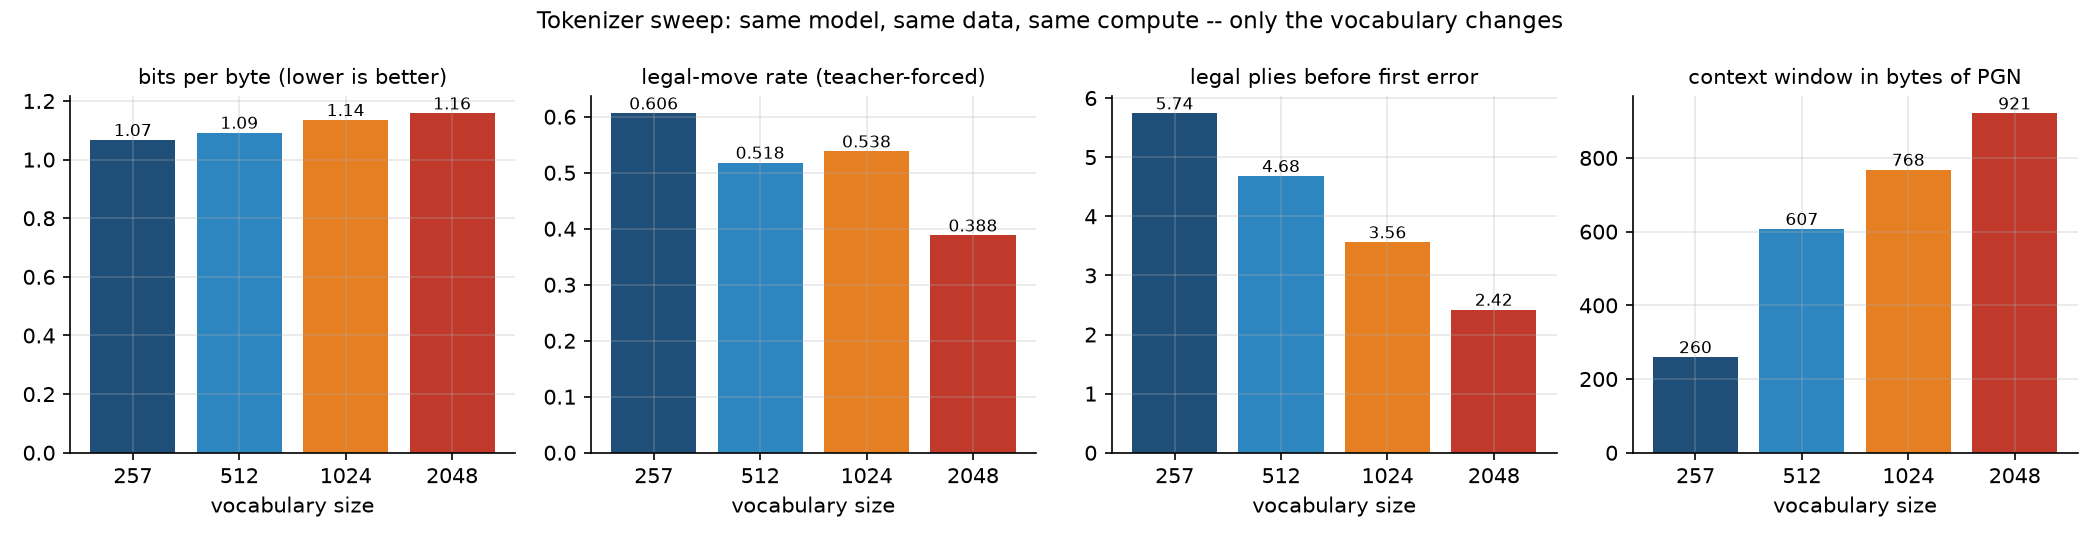
\includegraphics[width=0.98\textwidth]{../figures/fig2_sweep_summary.png}}{\typeout{Missing figure: fig2_sweep_summary.png}}
\caption{Summary of the four-vocabulary sweep under identical model architecture and compute: validation bits per byte, teacher-forced legal-move rate, mean consecutive legal plies in self-play, and effective context window in bytes of PGN.}
\label{fig:sweep-summary}
\end{figure}

Two mechanisms explain this inversion. First, in a fixed-step regime ($5{,}000$ updates $\times$ $32 \times 256 = 4.10 \times 10^7$ tokens), each individual token ID in a $2048$-token vocabulary receives nearly an order of magnitude fewer gradient updates than the $\sim 45$ active ASCII characters in the $257$-token model, leaving rare compound tokens under-trained. Second, unconstrained BPE merges frequently cross syntactic boundaries in PGN: inspection of $\mathcal{V}_{2048}$ reveals tokens such as \texttt{"8 4"}, \texttt{"5.Rc"}, and \texttt{".Rd1 R"} that fuse move numbers, piece letters, and spaces. Whereas the byte-level model always sees the compositional structure of a move (piece $\to$ file $\to$ rank), the BPE models must learn separate embeddings for the same chess move depending on which move number or capture symbol preceded it.

\subsection{Syntactic and state-dependent rule acquisition}
\label{sec:res-legality}

As shown in Table~\ref{tab:legality} and Figure~\ref{fig:legal-phase}, the byte-level model ($V=257$) achieves a $60.6\%$ teacher-forced legal-move rate across all game phases and matches the exact grandmaster move played in the test game $20.6\%$ of the time. When prompted with the first $10$ plies of a test game and left to play both sides on its own, it strings together an average of $5.74$ consecutive legal plies before committing its first illegal move.

\begin{table}[htbp]
\centering
\caption{Legal-move generation and exact grandmaster move match on held-out test games ($500$ teacher-forced positions; $50$ free-running rollouts from ply $10$).}
\label{tab:legality}
\medskip
{\footnotesize\setlength{\tabcolsep}{4.5pt}
\begin{tabular}{@{}rrrrrrr@{}}
\toprule
Vocab $V$ & Overall legal & Exact match & Opening ($<20$) & Middlegame ($20$--$59$) & Endgame ($60+$) & Free legal plies \\
\midrule
$257$  & $\mathbf{0.606}$ & $\mathbf{0.206}$ & $\mathbf{0.856}$ & $0.514$ & $\mathbf{0.465}$ & $\mathbf{5.74}$ \\
$512$  & $0.518$ & $0.150$ & $0.732$ & $0.450$ & $0.380$ & $4.68$ \\
$1024$ & $0.538$ & $0.126$ & $0.752$ & $\mathbf{0.518}$ & $0.318$ & $3.56$ \\
$2048$ & $0.388$ & $0.108$ & $0.549$ & $0.349$ & $0.264$ & $2.42$ \\
\bottomrule
\end{tabular}
}
\end{table}

\begin{figure}[htbp]
\centering
\IfFileExists{../figures/fig3_legal_by_phase.png}{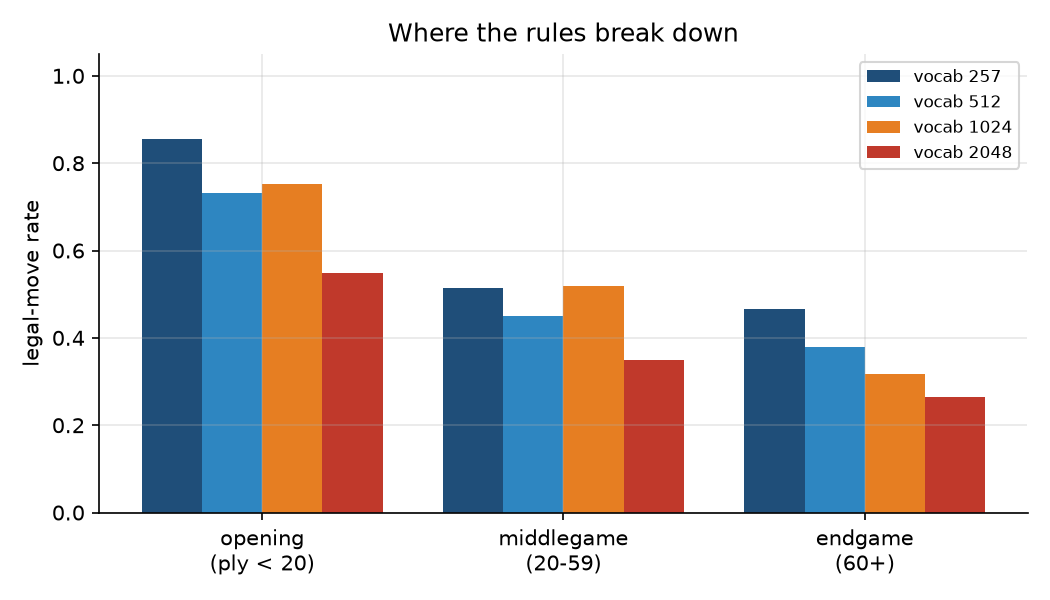
\includegraphics[width=0.75\textwidth]{../figures/fig3_legal_by_phase.png}}{\typeout{Missing figure: fig3_legal_by_phase.png}}
\caption{Teacher-forced legal-move rate broken down by game phase: opening ($\text{ply} < 20$), middlegame ($20 \le \text{ply} < 60$), and endgame ($\text{ply} \ge 60$). Legality is high in standard opening book lines and drops in the middlegame and endgame where legality requires tracking long-range piece movement and pinned pieces.}
\label{fig:legal-phase}
\end{figure}

Breaking legality down by game phase exposes the boundary between memorization and state tracking. In the opening ($\text{ply} < 20$), where grandmaster games follow well-trodden book lines (such as the Ruy Lopez \texttt{1.e4 e5 2.Nf3 Nc6 3.Bb5 a6}), the $V=257$ model produces a legal move $85.6\%$ of the time. In the middlegame ($20$--$59$ plies) and endgame ($60+$ plies), practically every position is unique to the test set; legality drops to $51.4\%$ and $46.5\%$, respectively. Notably, the $V=257$ model still outperforms all larger vocabularies in the endgame ($46.5\%$ vs.\ $26.4\%$ at $V=2048$) even though its $260$-byte context window truncates the early opening moves once a game passes ply ${\sim}20$.

\subsection{Emergent board state: linear probing across depth and squares}
\label{sec:res-probes}

Table~\ref{tab:probes} and Figure~\ref{fig:board-probe} report the accuracy of $64$-head linear probes trained to decode the board state from the residual stream $h^{(\ell)}_{\tau(k)}$ at each layer $\ell \in \{0, \dots, 5\}$. Across all four vocabularies, a consistent depth profile emerges:
\begin{enumerate}
\item At layer $\ell=0$ (the raw token embedding immediately after move $k$), probe accuracy ($65.0\%$--$69.0\%$ relative) is nearly indistinguishable from an untrained random network ($64.6\%$--$66.3\%$), because $h^{(0)}_{\tau(k)}$ contains only the identity of the single token that finished move $k$.
\item Across attention blocks $\ell = 1, 2, 3, 4$, overall relative board accuracy rises to $72.6\%$--$73.1\%$ ($72.8\%$--$73.5\%$ in absolute coordinates), gaining $+7.6$ to $+9.6$ percentage points over the per-square majority baseline ($63.5\%$).
\item On \emph{occupied squares}---the strict test of whether the probe knows where pieces actually sit rather than merely predicting empty squares---the trained models reach $33.8\%$--$35.8\%$ relative accuracy ($35.8\%$--$37.8\%$ absolute), more than doubling the untrained random-projection baseline ($8.3\%$--$14.4\%$) and exceeding the majority baseline ($2.7\%$) by a factor of $13\times$.
\item At the final layer $\ell=5$, board-probe accuracy drops across every vocabulary (for $V=257$, occupied accuracy falls from $33.8\%$ at layer $2$ to $25.0\%$ at layer $5$), reflecting the specialization of the pre-logit representation toward predicting the next character rather than maintaining the full board state.
\end{enumerate}

\begin{table}[htbp]
\centering
\caption{Linear board-state probe accuracy ($64$ squares $\times$ $13$ classes) on $11{,}656$ held-out test positions, comparing the best transformer layer against an untrained random-weight network and the per-square majority baseline.}
\label{tab:probes}
\medskip
{\footnotesize\setlength{\tabcolsep}{4.5pt}
\begin{tabular}{@{}rrrrrrrr@{}}
\toprule
 & \multicolumn{4}{c}{Relative board ($13$ classes)} & \multicolumn{3}{c}{Absolute board ($13$ classes)} \\
\cmidrule(lr){2-5} \cmidrule(lr){6-8}
Vocab $V$ & Best layer & Trained & Untrained & Occupied (tr / un) & Best layer & Trained & Occupied (tr / un) \\
\midrule
$257$  & $2$ & $0.726$ & $0.650$ & $0.338$ / $0.143$ & $2$ & $0.728$ & $0.358$ / $0.194$ \\
$512$  & $4$ & $\mathbf{0.731}$ & $0.663$ & $\mathbf{0.358}$ / $0.144$ & $3$ & $\mathbf{0.735}$ & $\mathbf{0.377}$ / $0.197$ \\
$1024$ & $4$ & $0.727$ & $0.652$ & $0.344$ / $0.106$ & $4$ & $0.734$ & $0.376$ / $0.159$ \\
$2048$ & $3$ & $0.726$ & $0.646$ & $0.341$ / $0.083$ & $4$ & $\mathbf{0.735}$ & $0.375$ / $0.139$ \\
\midrule
Majority & --- & \multicolumn{2}{c}{$0.635$} & $0.027$ & --- & $0.663$ & $0.165$ \\
\bottomrule
\end{tabular}
}
\end{table}

\begin{figure}[htbp]
\centering
\IfFileExists{../figures/fig4_board_probe_by_layer.png}{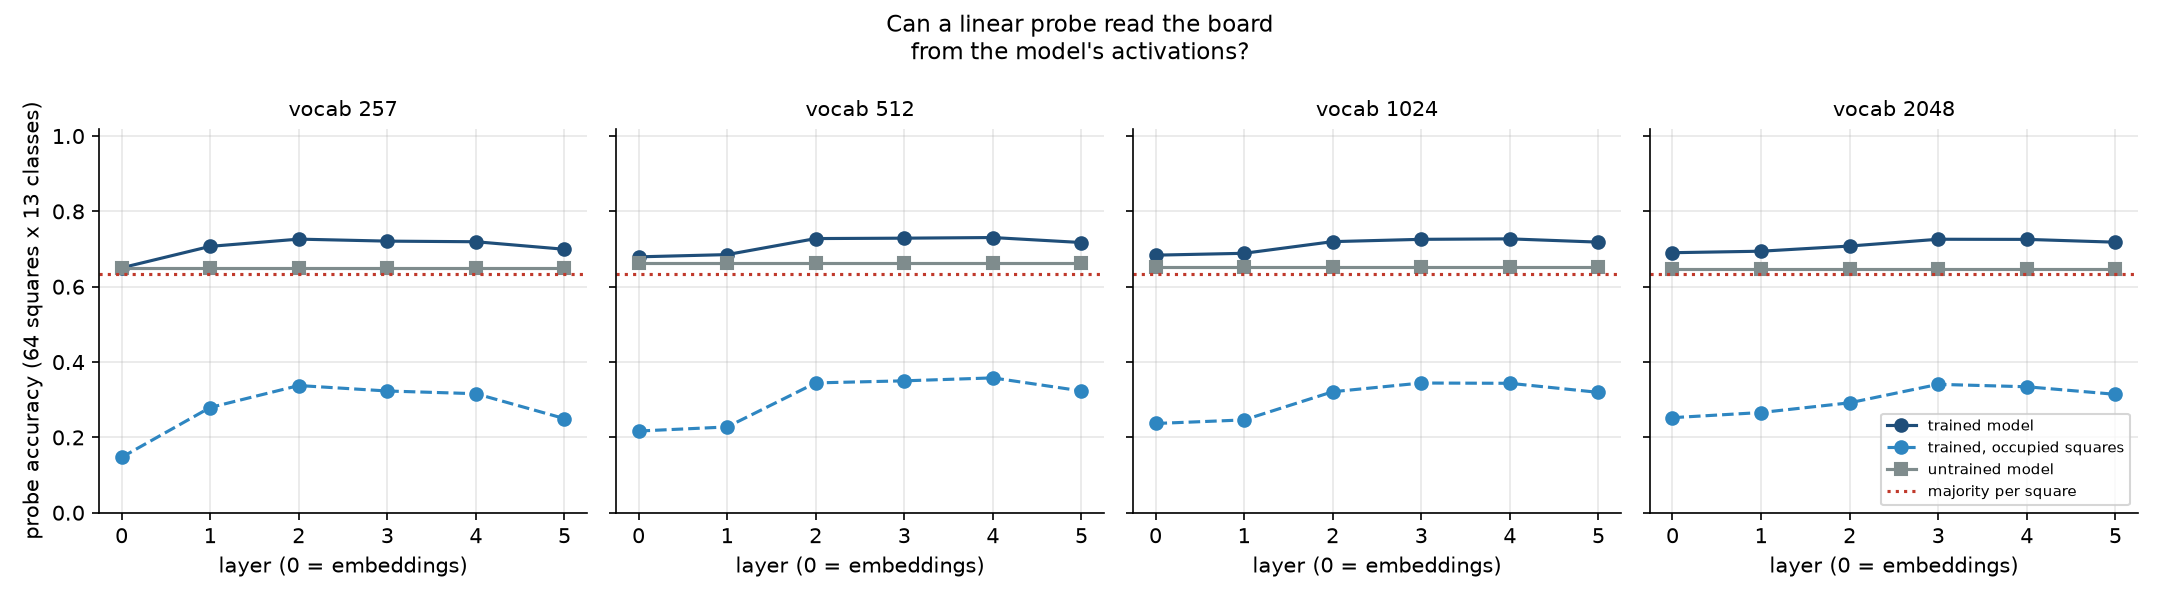
\includegraphics[width=0.98\textwidth]{../figures/fig4_board_probe_by_layer.png}}{\typeout{Missing figure: fig4_board_probe_by_layer.png}}
\caption{Linear probe accuracy for reconstructing the $64$-square relative board state across layers $\ell \in \{0, \dots, 5\}$ for each vocabulary size. Solid dark blue: all $64$ squares on the trained model; dashed light blue: occupied squares only; solid gray: identical probe trained on an untrained copy of the model; dotted red: per-square majority class.}
\label{fig:board-probe}
\end{figure}

Figure~\ref{fig:square-heatmap} displays the spatial distribution of probe accuracy across the $8\times 8$ board at layer $4$ of the $V=512$ model. Accuracy is highest ($81\%$--$86\%$) on the wing squares of the fourth and fifth ranks (\texttt{a4}, \texttt{b4}, \texttt{g4}, \texttt{h4}, \texttt{a5}, \texttt{b5}, \texttt{g5}, \texttt{h5}), which are empty across most of a game, and on the corner rook and castled king squares (\texttt{a1}, \texttt{h1}, \texttt{a8}, \texttt{h8}, $81\%$--$84\%$). Accuracy is lowest ($62\%$--$64\%$) in the central battleground (\texttt{d4}, \texttt{e4}, \texttt{d5}, \texttt{e5}, \texttt{c3}, \texttt{f3}, \texttt{c6}, \texttt{f6}), where pieces are repeatedly exchanged and occupancy flips several times per game.

\begin{figure}[htbp]
\centering
\IfFileExists{../figures/fig6_square_accuracy.png}{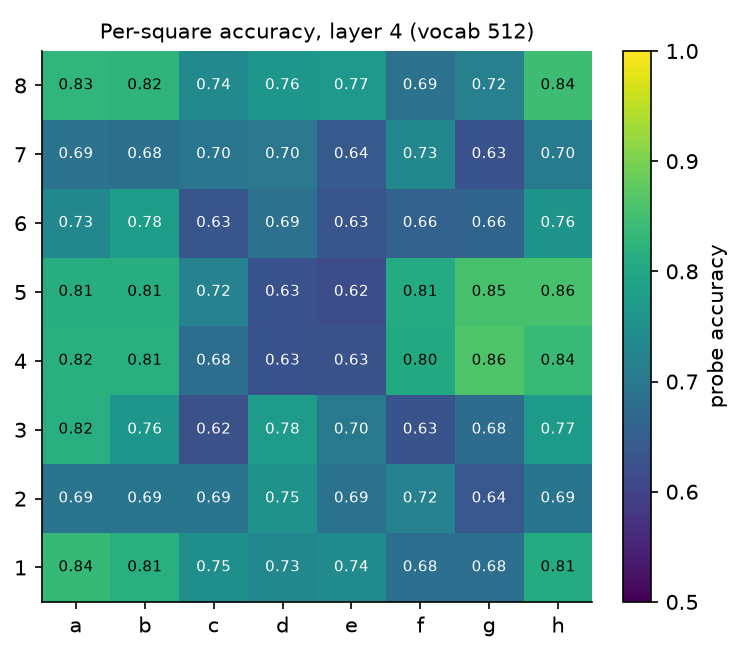
\includegraphics[width=0.58\textwidth]{../figures/fig6_square_accuracy.png}}{\typeout{Missing figure: fig6_square_accuracy.png}}
\caption{Per-square linear probe accuracy across the $8\times 8$ chessboard at layer $4$ ($V=512$, relative board encoding). Central squares (\texttt{d4}, \texttt{e4}, \texttt{d5}, \texttt{e5}) and knight development squares (\texttt{c3}, \texttt{f3}, \texttt{c6}, \texttt{f6}) experience the highest turnover of captures and exchanges and are hardest for a $64$-dimensional linear subspace to track.}
\label{fig:square-heatmap}
\end{figure}

\subsection{Outcome prediction and the zero-shot tokenization bias}
\label{sec:res-outcome}

Table~\ref{tab:outcome} and Figure~\ref{fig:outcome} compare five methods for predicting the three-way game outcome (\texttt{1-0}, \texttt{0-1}, \texttt{1/2-1/2}) from a game prefix. On the held-out test set, outcomes are fairly balanced ($35.3\%$ White wins, $29.2\%$ Black wins, $35.5\%$ draws; majority baseline accuracy $35.5\%$, macro-$F_1 = 0.175$). A linear classifier using only the current board's material balance reaches $42.5\%$ accuracy ($F_1 = 0.380$), rising steeply from $36.6\%$ in the first quarter of the game (where material is almost always equal) to $53.3\%$ in the final quarter. Adding player Elo difference lifts accuracy across the entire game to $55.3\%$ ($F_1 = 0.550$), even in the opening quartile ($54.1\%$).

\begin{table}[htbp]
\centering
\caption{Three-way game outcome prediction (\texttt{1-0}, \texttt{0-1}, \texttt{1/2-1/2}) on held-out test games across game-length quartiles ($0$--$25\%$, $25$--$50\%$, $50$--$75\%$, $75$--$100\%$).}
\label{tab:outcome}
\medskip
{\footnotesize\setlength{\tabcolsep}{4.5pt}
\begin{tabular}{@{}lrrrrrr@{}}
\toprule
Method & Overall acc & Macro-$F_1$ & $0$--$25\%$ & $25$--$50\%$ & $50$--$75\%$ & $75$--$100\%$ \\
\midrule
Majority class baseline & $0.355$ & $0.175$ & $0.357$ & $0.365$ & $0.361$ & $0.338$ \\
Material balance & $0.425$ & $0.380$ & $0.366$ & $0.373$ & $0.422$ & $0.533$ \\
Material + Elo difference & $\mathbf{0.553}$ & $\mathbf{0.550}$ & $\mathbf{0.541}$ & $\mathbf{0.534}$ & $\mathbf{0.560}$ & $\mathbf{0.577}$ \\
\midrule
Activation probe ($V=257$, layer $5$) & $0.386$ & $0.305$ & $0.366$ & $0.398$ & $0.388$ & $0.392$ \\
Activation probe ($V=512$, layer $5$) & $0.397$ & $0.351$ & $0.365$ & $0.390$ & $0.406$ & $0.423$ \\
Activation probe ($V=1024$, layer $4$) & $0.396$ & $0.350$ & $0.370$ & $0.375$ & $0.423$ & $0.414$ \\
Activation probe ($V=2048$, layer $3$) & $0.394$ & $0.343$ & $0.366$ & $0.399$ & $0.404$ & $0.404$ \\
\midrule
Zero-shot LM ($V=257$) & $0.365$ & $0.355$ & $0.323$ & $0.361$ & $0.368$ & $0.410$ \\
Zero-shot LM ($V \in \{512, 1024, 2048\}$) & $0.341$ & $0.169$ & $0.365$ & $0.318$ & $0.357$ & $0.324$ \\
\bottomrule
\end{tabular}
}
\end{table}

\begin{figure}[htbp]
\centering
\IfFileExists{../figures/fig5_outcome_prediction.png}{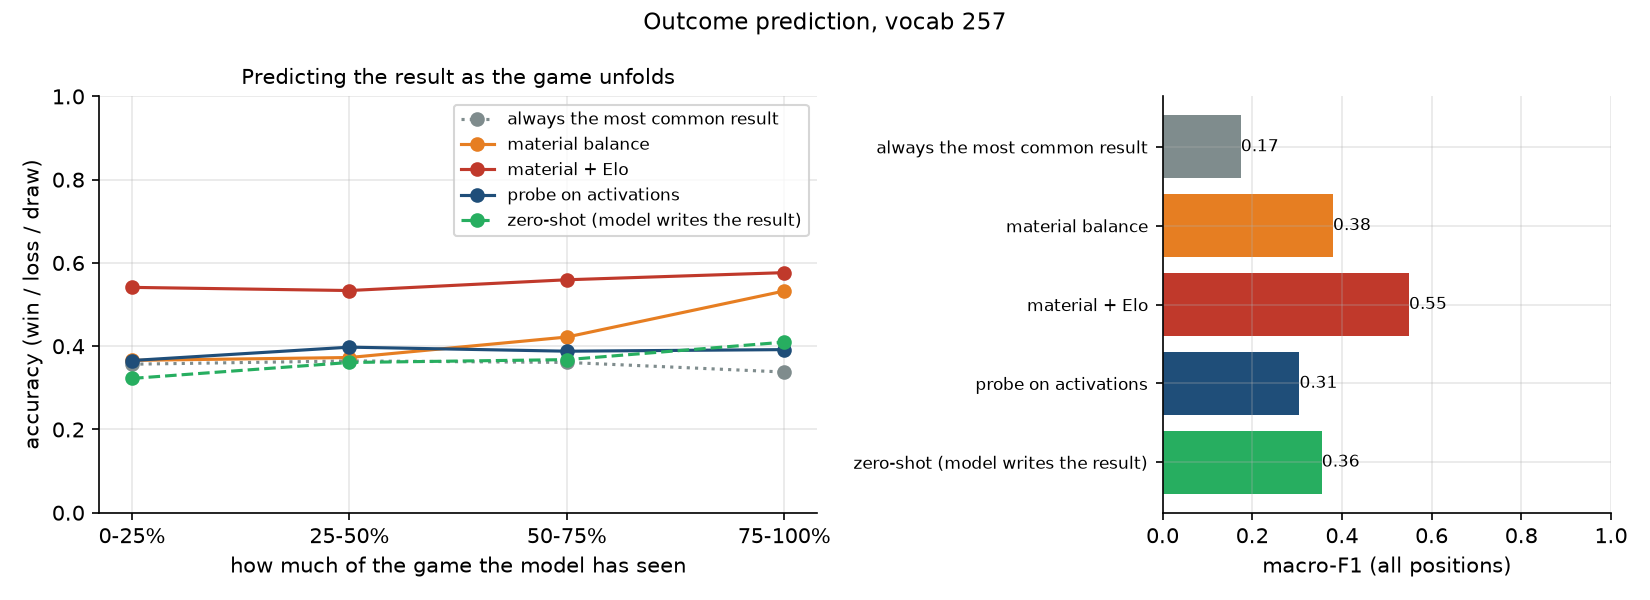
\includegraphics[width=0.95\textwidth]{../figures/fig5_outcome_prediction.png}}{\typeout{Missing figure: fig5_outcome_prediction.png}}
\caption{Outcome prediction accuracy across game-progress quartiles (left) and overall macro-$F_1$ (right) for $V=257$. While both the activation probe and byte-level zero-shot scoring improve toward the end of the game ($41.0\%$ zero-shot accuracy in the final quartile), neither approaches the material-balance ($53.3\%$) or material-plus-Elo ($57.7\%$) baselines.}
\label{fig:outcome}
\end{figure}

By contrast, linear probes on the transformer's residual stream achieve only $38.6\%$--$39.7\%$ accuracy ($F_1 = 0.305$--$0.351$), rising modestly to $42.3\%$ in the final quarter of the game for $V=512$. Zero-shot scoring---appending \texttt{" 1-0"}, \texttt{" 0-1"}, or \texttt{" 1/2-1/2"} to a prefix and comparing $\ln P(\text{result} \mid \text{prefix})$---reveals an instructive negative result:
\begin{itemize}
\item For the byte-level model ($V=257$), zero-shot scoring achieves macro-$F_1 = 0.355$ overall and rises monotonically with game progress from $32.3\%$ in the opening quartile to $41.0\%$ in the final quartile, confirming a weak end-of-game signal.
\item For every BPE model ($V \in \{512, 1024, 2048\}$), zero-shot scoring collapses to macro-$F_1 = 0.169$ ($34.1\%$ accuracy), predicting \texttt{1-0} on virtually $100\%$ of mid-game prefixes. Inspection of the BPE merge tables explains why: in $\mathcal{V}_{512}$, $\mathcal{V}_{1024}$, and $\mathcal{V}_{2048}$, the string \texttt{" 1-0"} is tokenized into $2$ tokens (\texttt{[' 1', '-0']}) or merged directly with the preceding move digit (\texttt{'8 1'}, \texttt{'-0'}), whereas \texttt{" 0-1"} is split into $3$--$4$ tokens (\texttt{[' ', '0', '-', '1']}). Because a game termination string is out of distribution in the middle of an ongoing game, every individual result token incurs a large log-probability penalty (${\sim}-10$ to $-25$ nats); summing over $2$ tokens rather than $3$ gives \texttt{1-0} a constant $+25$ to $+45$ nat advantage regardless of the board position.
\end{itemize}

\section{Discussion and Limitations}
\label{sec:discussion}

\paragraph{Capacity bottleneck ($d_{\mathrm{model}}=64$).} The clearest limitation of the present models is width. Representing a $64$-square board over $13$ piece classes requires packing $64$ categorical variables into a single $64$-dimensional vector $h^{(\ell)}_t \in \mathbb{R}^{64}$---literally one real dimension per chessboard square. Previous work demonstrating near-perfect linear board probes in chess transformers \citep{toshniwal2022chess,karvonen2024chess} used models with $d_{\mathrm{model}} \in [512, 768]$ and $8$--$12$ layers (${\sim}25\mathrm{M}$--$85\mathrm{M}$ parameters), roughly two orders of magnitude larger than our CSE 142 course architecture. That a $344\mathrm{K}$-parameter, $64$-dimensional model nevertheless recovers $35.8\%$ of occupied squares linearly ($13\times$ the majority baseline and $2.5\times$ an untrained network) shows that world-state tracking begins to emerge even in tiny transformers, but saturates quickly when residual-stream width equals the number of board squares.

\paragraph{Context truncation vs.\ BPE boundary corruption.} In principle, byte-level tokenization ($V=257$) suffers from a severe handicap in chess: a $256$-byte context window holds only $\sim 18$--$20$ plies, so by move $25$ the model can no longer see where the pieces moved in the opening. Yet $V=257$ still beats $V=512, 1024, 2048$ on endgame legality and matches them on board-probe accuracy. This indicates that for small models, preserving clean, shift-invariant sub-move boundaries (so \texttt{Nf3} is always tokenized the same way) matters more than extending the context horizon via unrestricted BPE merges. A natural improvement for future work is \emph{pre-tokenized} or whitespace-restricted BPE (as in GPT-2), forbidding merges across spaces and move-number periods so that vocabulary compression does not corrupt move boundaries.

\paragraph{Why outcome prediction fails without board supervision.} In grandmaster chess, most games are decided by subtle positional advantages or single-ply tactical blunders before resignations occur, while material remains balanced for most of the game. Because the PGN movetext contains no intermediate evaluation annotations and no player Elo headers, a next-token predictor trained only on moves has almost no gradient signal connecting mid-game positions to the final $3$ bytes (\texttt{1-0}, \texttt{0-1}, \texttt{1/2-1/2}) until the final few moves before resignation or checkmate.

\section{References}
\label{sec:references}

\bibliographystyle{plainnat}
\bibliography{refs}

\end{document}
